\section{Data Analysis} \label{data}
The data is split into three main parts: \textit{demographics} (before playing the game), \textit{mid-questionnaire} (while playing the game) and \textit{post-questionnaire} (after playing the game). The mid-questionnaire consists of two parts. In the first part, participants described the game feel in their own words. In the second part, participants rated the game feel on pre-defined words using Likert scales. The post-questionnaire is about game feel in general. The following analyzes the data from the three parts.

\subsection{Demographics}
As stated previously, the game was mainly shared on gaming websites. At the time of writing, 274 participants have played the game. Tables \ref{table:demographics1} and \ref{table:demographics2} show demographical data about the participants. Most of the participants rated themselves quite experienced with both playing videogames in general and playing 2D platforming games. The average death count was 5, the average framerate 59.7 FPS and the average time spent per level was 61 seconds/level.

\begin{table} \centering
\small
\caption{Demographics data 1.}
\label{table:demographics1}
\renewcommand{\arraystretch}{1.2}
\begin{tabular}{cccc}
\toprule
\textbf{Platform} & Windows Web: & Windows Exe: & Mac Web: \\
                  & 55.2\%      & 30.7\%      & 14.1\%  \\
\textbf{Gender}   & Male:        & Female:      & Other:   \\
                  & 93.6\%      & 5.7\%       & 0.7\%   \\
\textbf{Age}      & Male:     & Female:            & Other:        \\
                  & 24.6 years  & 23.9 years           & 25 years        \\
\bottomrule
\end{tabular}
\end{table}

\begin{table} \centering
\small
\caption{Demographics data 2.}
\label{table:demographics2}
%\renewcommand{\arraystretch}{1.2}
\begin{tabular}{lcc}
\toprule
\textbf{Regions}                      &                & \textbf{}               \\ 
\textit{Europe}                      & 70.6\%         &                         \\
\textit{Americas}                    & 26.7\%         &                         \\
\textit{Asia}                        & 1.9\%          &                         \\
\textit{Oceania}                     & 0\%            &                         \\
\textit{Africa}                      & 0.6\%          &                         \\
\textit{Other}                       & 0.2\%          &                         \\
\textbf{Experience with...} & \textbf{Videogames} & \textbf{2D platformers} \\
\textit{1 (none)}                           & 0\%            & 0\%                     \\
\textit{2}                           & 0\%            & 3.1\%                   \\ 
\textit{3}                           & 0.6\%          & 10.1\%                  \\
\textit{4}                           & 4\%            & 14.1\%                  \\ 
\textit{5}                           & 9.6\%          & 23.2\%                  \\ 
\textit{6}                           & 22.5\%         & 16.9\%                  \\
\textit{7 (a lot)}                           & 63.3\%         & 32.6\%                  \\
\bottomrule
\end{tabular}
\end{table}

As stated in Section \ref{latinSection}, ideally there should be an equal amount of participants in each of the four Latin square sequences. However, as shown in Table \ref{table:latinSequenceNumber}, this is not the case. This might be due to players either quitting halfway, or that participants for some reason lost their Internet connection while trying to access the current Latin square number (in this case, the sequence was chosen randomly). Each time a participant collected three stars and answered the mid-questionnaire, data was logged. In total, 701 data logs were collected. Figure \ref{fig:retention} illustrates the retention rate of the participants.

Figure \ref{fig:overallDistribution} shows the overall distribution of the acceleration/deceleration combinations that participants experienced. As stated previously, the time intervals were either \textit{fast} (1-240 ms) or \textit{slow} (241-1500 ms). Since the lengths of the intervals are not of equal size, neither are the distribution, as shown in the figure. A way to counter this would be to divide the \textit{slow} category into multiple smaller intervals of equal sizes, but this would also affect the number of possible sequences and Latin squares.

\begin{table} \centering
%\small
\caption{The number of data entries in each of the four Latin square sequences.}
\label{table:latinSequenceNumber}
\begin{tabular}{cc}
\toprule
& \textbf{Number of data entries}\\
\midrule
\textbf{Sequence 1} & 190\\
\textbf{Sequence 2} & 179\\
\textbf{Sequence 3} & 165\\
\textbf{Sequence 4} & 167\\
\bottomrule
\end{tabular}
\end{table}

\begin{figure}[htbp]
\centering
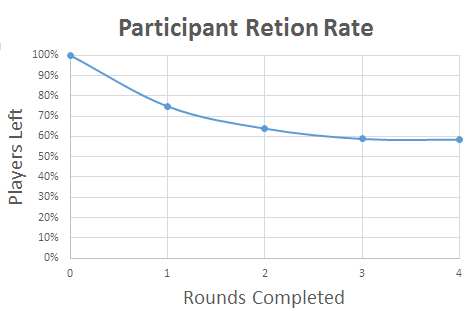
\includegraphics[width=0.4\textwidth]{Pics/retetionRate}
\caption{274 participants started the game, but not all completed the four rounds, presumably due to fatigue or boredom.}
\label{fig:retention}
\end{figure}

\subsection{Mid-questionnaire}
Whenever players collected three stars, they were met with a set of questions (see Figure \ref{fig:questionnaire}). In the first part, participants described the game feel in their own words, while in the second part they were asked to rate pre-defined words on a 7-point Likert scale (1 = \textit{not at all}; 7 = \textit{a lot}).

\begin{figure}[htbp]
\centering
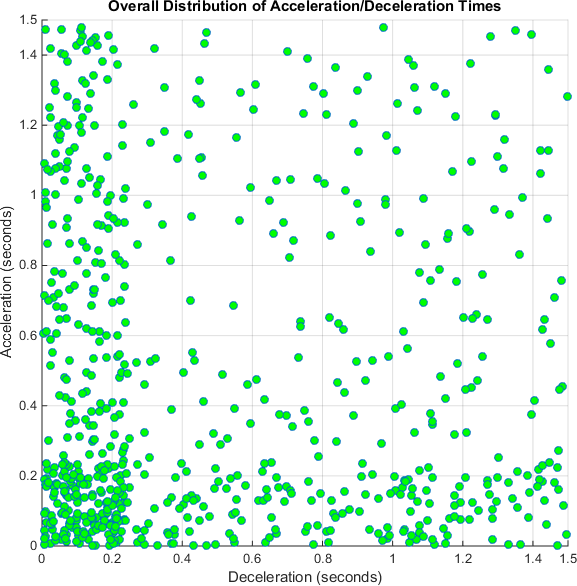
\includegraphics[width=0.7\columnwidth]{Pics/Classes/overall_distribution}
\caption{Scatter plot of all the different acceleration/deceleration combinations participants experienced.}
\label{fig:overallDistribution}
\end{figure}

\subsubsection{Describing Game Feel in Own Words}
Table \ref{table:mostWords} shows the 30 most commonly-used words that participants used to describe the game feel (both on ground and in air). Additionally, these words have manually, by the author, been put into one or more of following nine categories (see Figures \ref{fig:coding1} and \ref{fig:coding2}).
\begin{itemize}[noitemsep,nolistsep]
\item Single words or multiple words?
\item Basic or complex words? (basic words are root words that can stand on their own, e.g., \textit{heavy} and \textit{laggy}, whereas complex words consist of modifiers that somehow change the meaning of the root words, e.g., \textit{very fast} and \textit{a bit sluggish})
\item Did the words express anything about quality or opinion? (using words such as \textit{fun}, \textit{too fast}, \textit{very annoying} and \textit{unrealistic})
\item Did the words describe anything related to the difficulty?
\item Did the words use physical properties or make comparisons to anything from the real world? (\textit{like dragging through light mud}, using words such as \textit{force}, \textit{velocity} and \textit{momentum})
\item Did the words make comparisons to other games? (\textit{like Mario} or \textit{like Mega Man})
\item Did the words make comparisons to previous rounds of the game? (\textit{felt no difference from last game})
\end{itemize}

Note that a description can include words from multiple categories. The average word count was 5.4 words for ground description and 5.1 words for air description.

Interestingly, there were some participants who had problems feeling any difference between the four rounds. One participant kept writing \textit{``No difference at all"}. This participant was presented with the following four sequences [acceleration;deceleration]: \textbf{[0.03;0.07]}, \textbf{[0.3;0.78]}, \textbf{[1.0;0.2]}, \textbf{[0.1;0.4]}. Assuming that the system worked correctly, it seems odd that the participant could not feel any difference between the rounds.

Below are some selected quotes and their corresponding acceleration and deceleration values in square brackets (ascending order of acceleration values).
\begin{itemize}[noitemsep,nolistsep]
\item Grounded, wavy, skill-based, inertia, chunky \textbf{[0.03;0.66]}
\item It's okay fast. Not with an acceleration, just one constant speed (which maybe makes it easier to control but then again more boring to look at) \textbf{[0.05;0.21]}
\item Only goes where you want it to go. No physics \textbf{[0.05;0.07]}
\item Very responsive, felt ``right" \textbf{[0.06;0.03]}
\item Icy \textbf{[0.07;1.16]}
\item Super twitchy, ball moves right when you press keys \textbf{[0.09;0.14]}
\item Annoying, no fine control, noticeable input delay \textbf{[0.1;0.18]}
\item Very static. Actually easier once you're used to it, but less intuitive and fun \textbf{[0.22;0.49]}
\item Feels like you're rolling a big ball down a hill almost - it takes a bit of time to get going \textbf{[0.27;1.47]}
\item It feels really heavy and has a bit of after roll that adds a bit of reality feeling physics to it \textbf{[0.3;0.52]}
\item Like Super Mario (which is good) \textbf{[0.34;0.14]}
\item Heavy like a bowling ball, smooth \textbf{[0.38;0.74]}
\item Unrealistic, stiff. The fact that it stops on a dime, except when you press in the opposite direction feels odd \textbf{[0.52;0.07]}
\item The ball felt really good, and I liked that it didn't stop completely when I stopped pushing the button \textbf{[0.52;0.26]}
\item BAD!!! Not like a ball at all. It is confusing \textbf{[0.93;0.07]}
\item Extremely annoying and heavy. Way too slow acceleration and reaction time in change of direction was truly painful \textbf{[0.97;0.29]}
\item Slow, annoying, snappy \textbf{[1.0;0.03]}
\item Fast, but also slippery \textbf{[1.06;1.17]}
\item It controls like a truck with square wheels \textbf{[1.19;0.07]}
\item Lots of momentum, ball takes a while to accelerate and a while to decelerate \textbf{[1.22;1.29]}
\item Very slow to start, stopped really fast. Punishing to not ``give full throttle" \textbf{[1.24;0.09]}
\item Mechanical, sometimes ``jumps" forwards. No fine control \textbf{[1.3;1.1]}
\item Sluggish not fun \textbf{[1.31;0.77]}
\item Heavy and unpleasant as hell \textbf{[1.41;0.02]}
\item Felt like dragging through light mud with reasonable control \textbf{[1.41;0.12]}
\item Heavy, slow, unrealisticly heavy \textbf{[1.4;0.7]}
\item Sticks like glue \textbf{[1.47;0.01]}
\item Slow, heavy, poor acceleration \textbf{[1.47;0.97]}
\end{itemize}

Ostensibly, there are different opinions on what feels ``right". Obviously, some of the higher values yield more frustrating results, since there is a longer delay before the participant sees the result on the screen. Some participants tried to describe the feeling using words from the physical world, such as \textit{momentum}, \textit{acceleration} and \textit{friction}. Others expressed themselves whenever they felt that the controls were \textit{too heavy} or \textit{too unresponsive}. Some compared it to \textit{a heavy tank moving through mud}, while others critiqued that the movement was \textit{unrealistic} and \textit{didn't feel like a ball at all}. Some participants were eager to express how much \textit{easier} or \textit{difficult} the game was due to the controls, while others emphasized personal opinions, such as it feeling \textit{too fast} or \textit{not fun}.

\begin{table} \centering
\caption{The 30 most commonly-used words to describe the feel of the game (among the 701 data entries). Numbers in parenthesis indicate usage frequency. Common grammar words have been excluded.}
\label{table:mostWords}
\begin{tabular}{lll}
\toprule
heavy (165) & slow (132) & ball (122)\\
responsive (104) & fast (94) & like (90)\\
control (87) & very (83) & too (80)\\ 
easy (78) & momentum (61) & realistic (61)\\
sluggish (58) & floaty (58) & bit (54)\\
air  (52) & good (51) & unrealistic (51)\\
feels (50) & little (45) & hard (42)\\
felt (40) & fluid (39) & still (38)\\
ground (37) & jump (37) & same (36)\\
speed (35) & time (34) & stop (31)\\
\bottomrule
\end{tabular}
\end{table}

\begin{figure}[htbp]
\centering
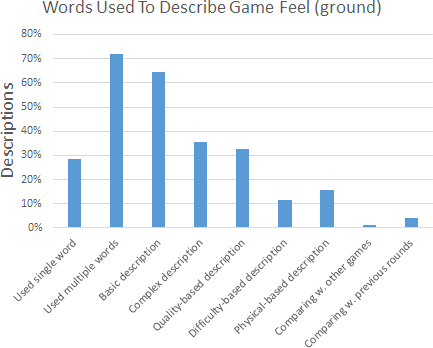
\includegraphics[width=\columnwidth]{Pics/coding1}
\caption{The different types of words participants used to describe the game feel on ground.}
\label{fig:coding1}
\end{figure}

\begin{figure}[htbp]
\centering
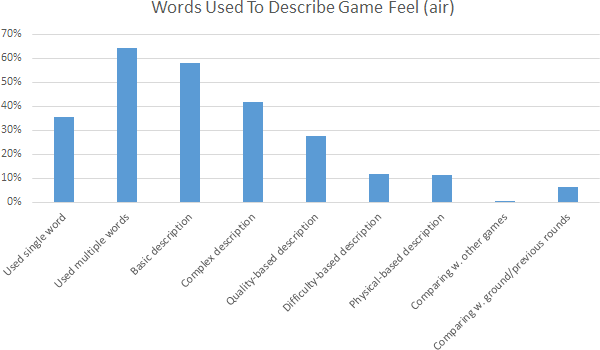
\includegraphics[width=\columnwidth]{Pics/coding2}
\caption{The different types of words participants used to describe the game feel in air.}
\label{fig:coding2}
\end{figure}

%\begin{figure*}[htbp]
%\centering
%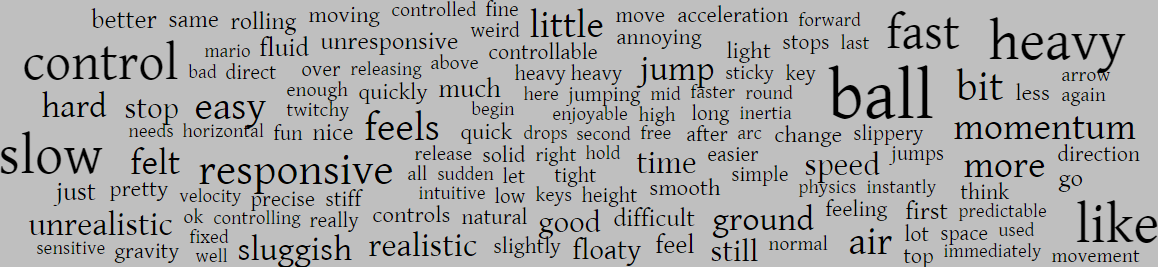
\includegraphics[width=1\textwidth]{Pics/wordcloud}
%\caption{The 130 most commonly-used words to describe the feel of the controls (both on ground and %in air). Bigger means a word has been used more frequently. Common words such as \textit{a}, %\textit{also}, \textit{and}, \textit{have}, \textit{could}, etc. have been excluded. Created with %WordItOut.com.}
%\label{fig:wordcloud}
%\end{figure*}

\subsubsection{Rating Game Feel with Pre-Defined Words}
Using a 7-point Likert scale, participants also rated the game feel on the following pre-defined terms.
\begin{itemize}[noitemsep,nolistsep]
\item Twitchy
\item Fluid
\item Stiff
\item Floaty
\item Responsive
\item Enjoyable
\item Difficult
\item How much they liked the controls
\item Frustration
\end{itemize}

\textbf{Looking at Acceleration and Deceleration Separately}\\
%One way to illustrate the responses is to plot the Likert ratings along the axes of either acceleration or deceleration, as shown in Figures \ref{fig:twitchy_both} \ref{fig:fluid_both}, \ref{fig:stiff_both}, \ref{fig:floaty_both} and \ref{fig:responsive_both}. Even though one might be able to spot some slight tendencies, 
Figure \ref{fig:correlationMatrix} shows the correlation matrix. Here, it is possible to spot a few tendencies, e.g., acceleration having a negative correlation with how \textit{twitchy}, \textit{fluid}, \textit{floaty} and \textit{responsive} the game felt. Meanwhile, deceleration has a positive correlation with how \textit{twitchy} and \textit{floaty} the game felt. However, this way of showing the data is not accurate, since it splits the acceleration and deceleration. The participants did not experience either in a vacuum; both were apparent when playing.

%\begin{figure*}[htbp]
%\centering
%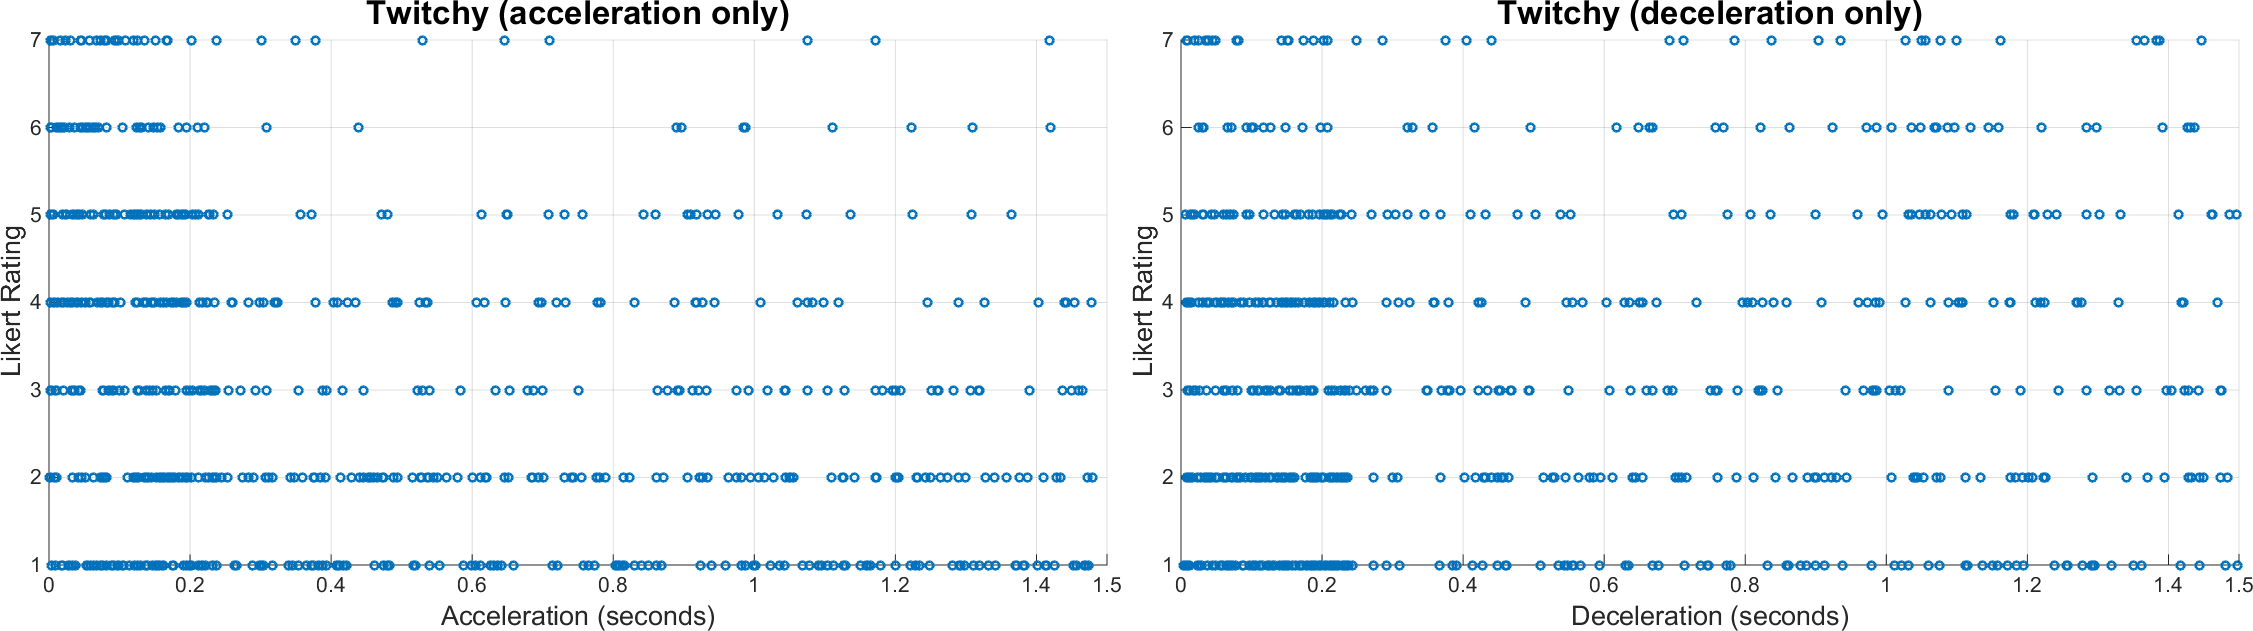
\includegraphics[width=0.95\textwidth]{Pics/Classes/twitchy_both}
%\caption{Looking at twitchy for acceleration and deceleration.}
%\label{fig:twitchy_both}
%\end{figure*}

%\begin{figure*}[htbp]
%\centering
%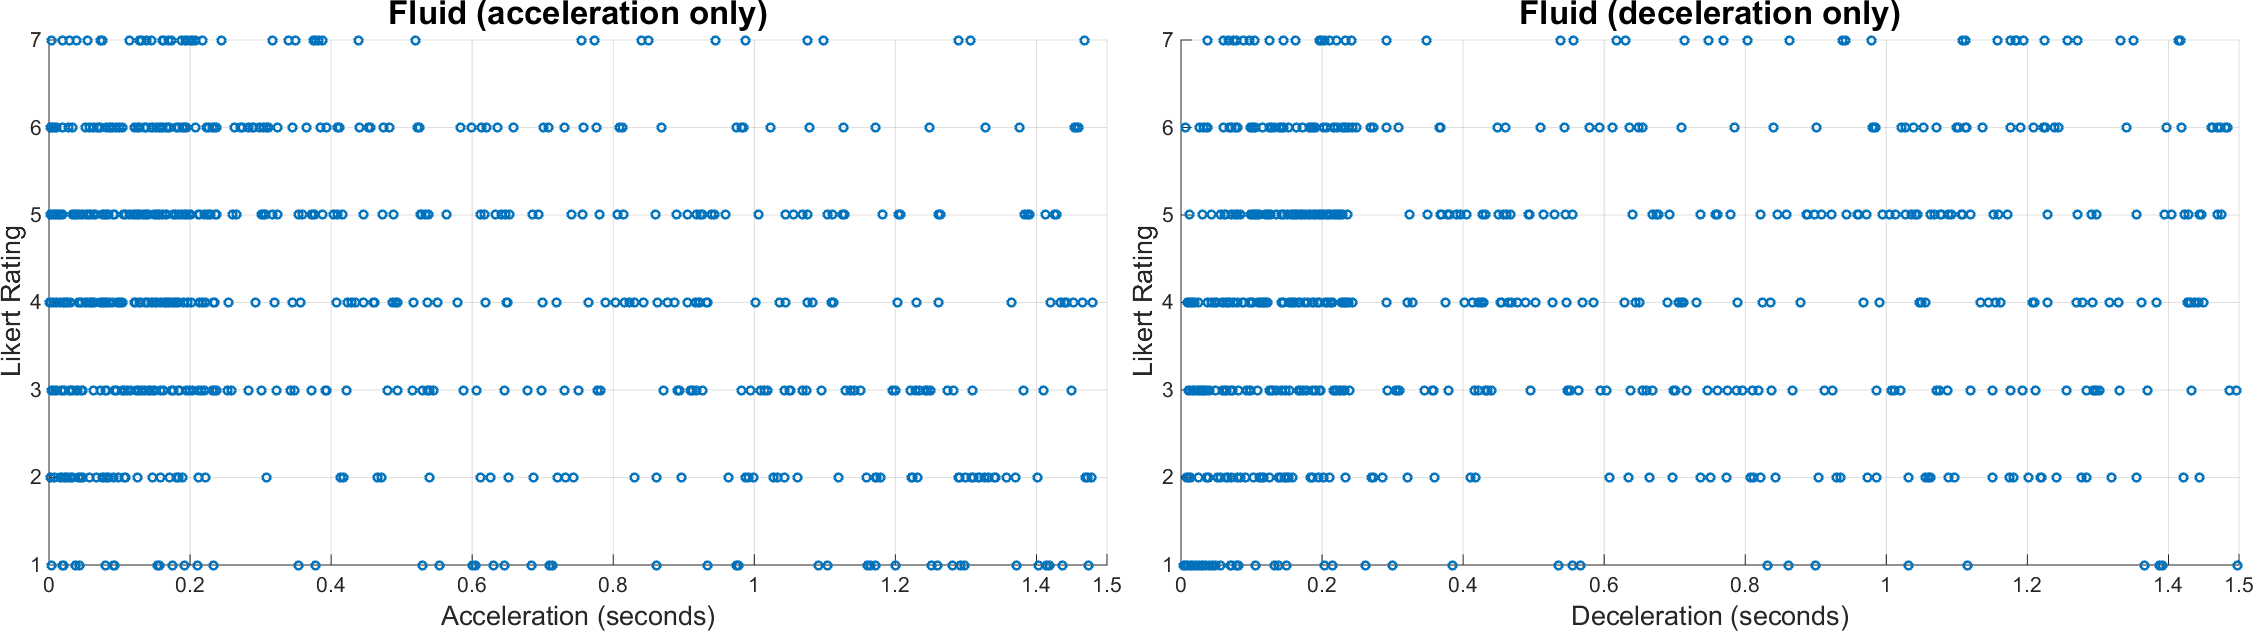
\includegraphics[width=0.95\textwidth]{Pics/Classes/fluid_both}
%\caption{Looking at fluid for acceleration and deceleration.}
%\label{fig:fluid_both}
%\end{figure*}

%\begin{figure*}[htbp]
%\centering
%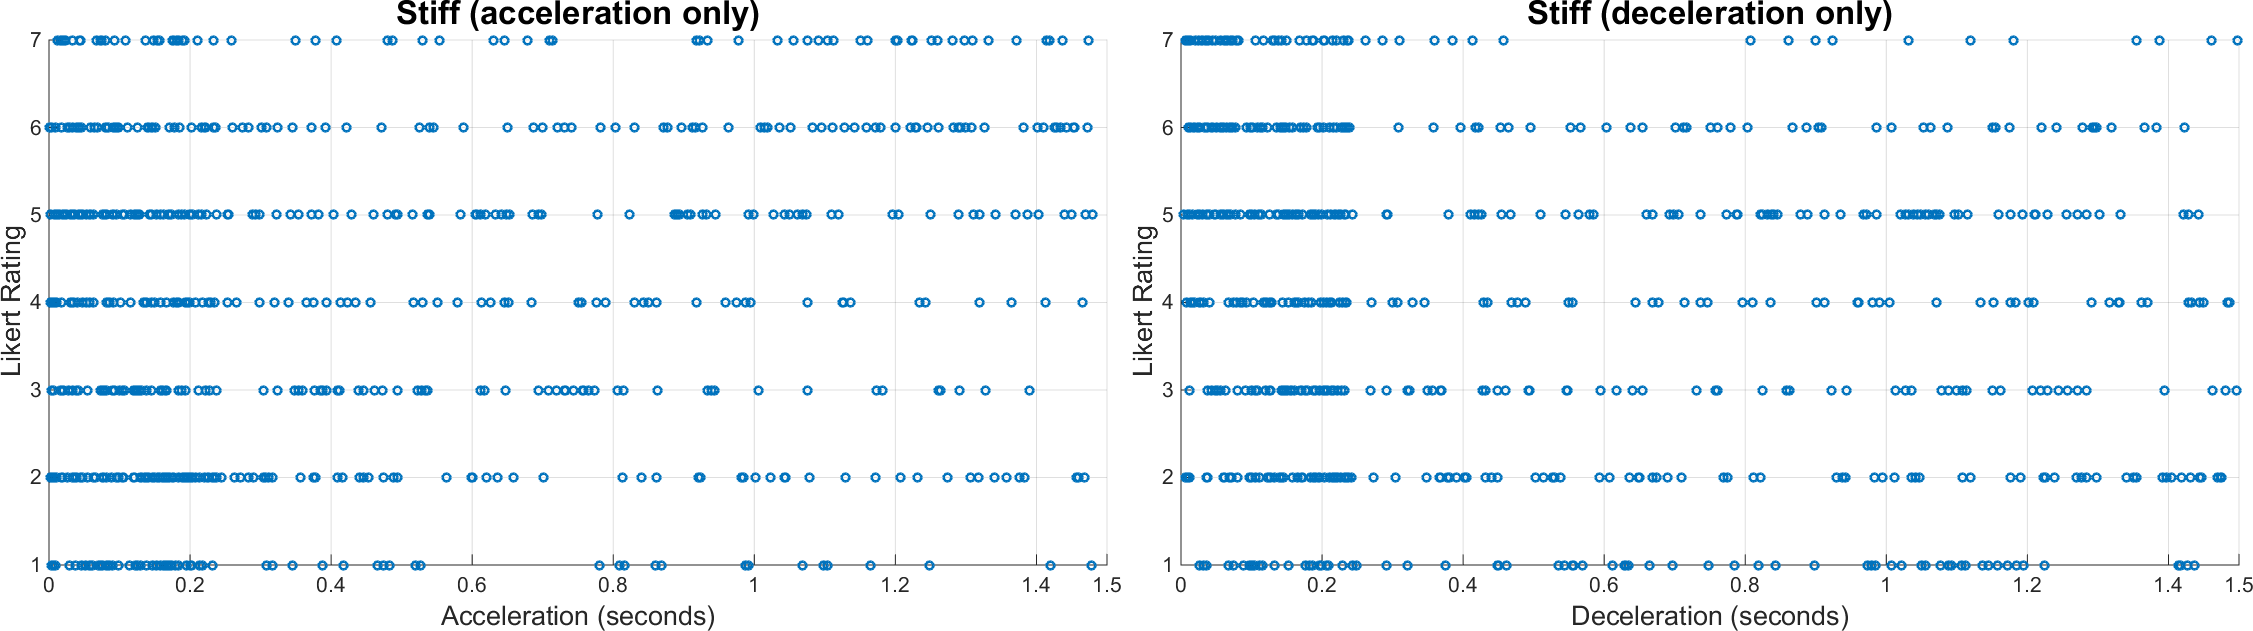
\includegraphics[width=0.95\textwidth]{Pics/Classes/stiff_both}
%\caption{Looking at stiff for acceleration and deceleration.}
%\label{fig:stiff_both}
%\end{figure*}

%\begin{figure*}[htbp]
%\centering
%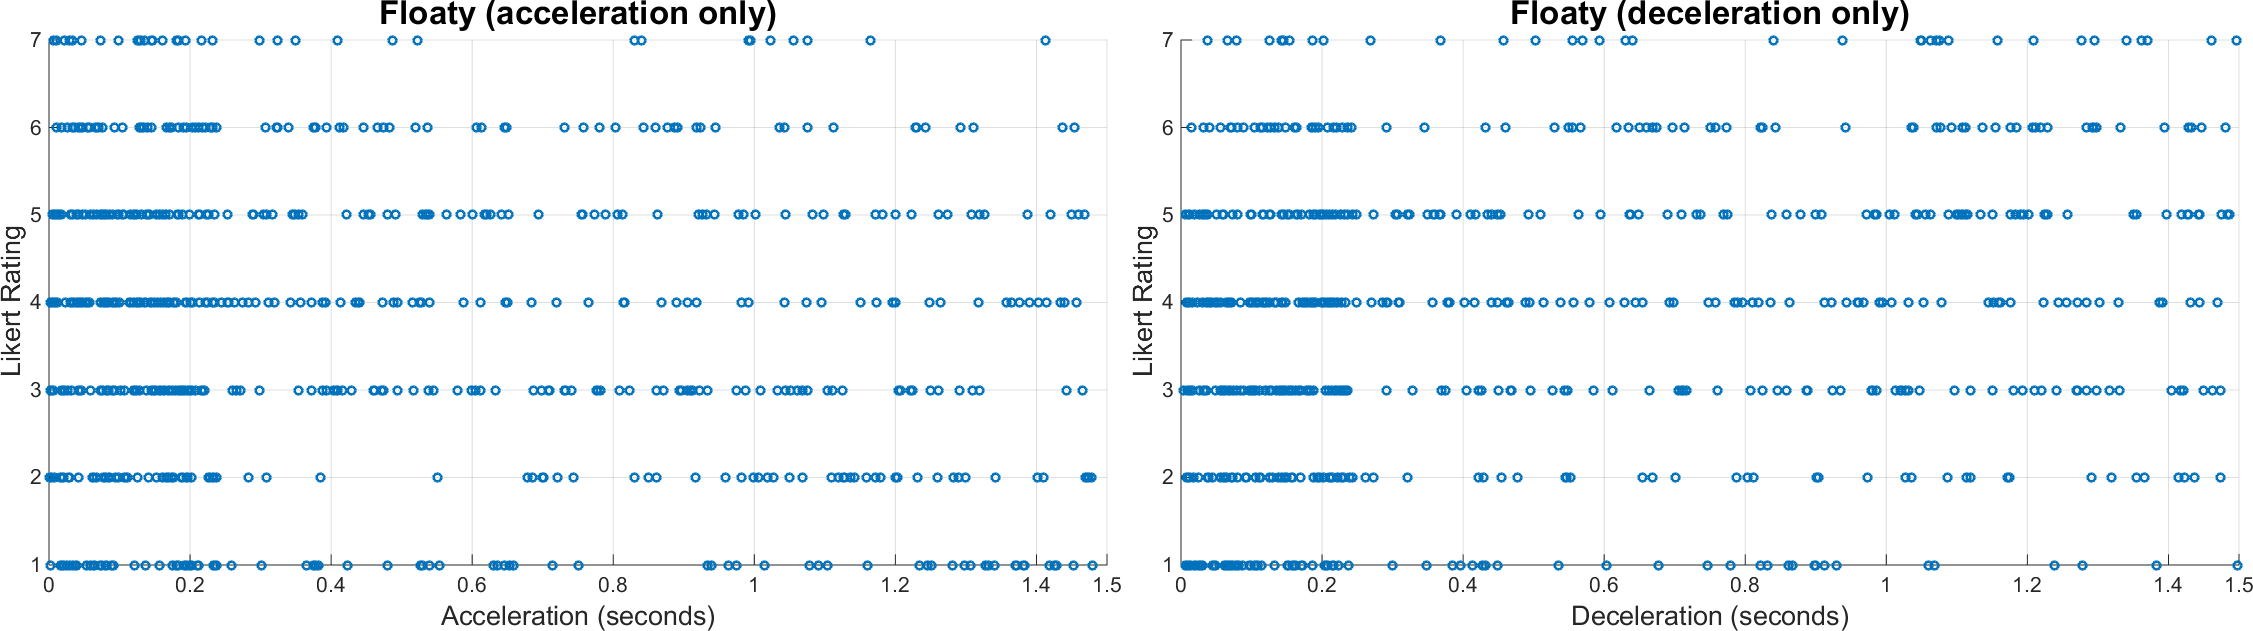
\includegraphics[width=0.95\textwidth]{Pics/Classes/floaty_both}
%\caption{Looking at floaty for acceleration and deceleration.}
%\label{fig:floaty_both}
%\end{figure*}

%\begin{figure*}[htbp]
%\centering
%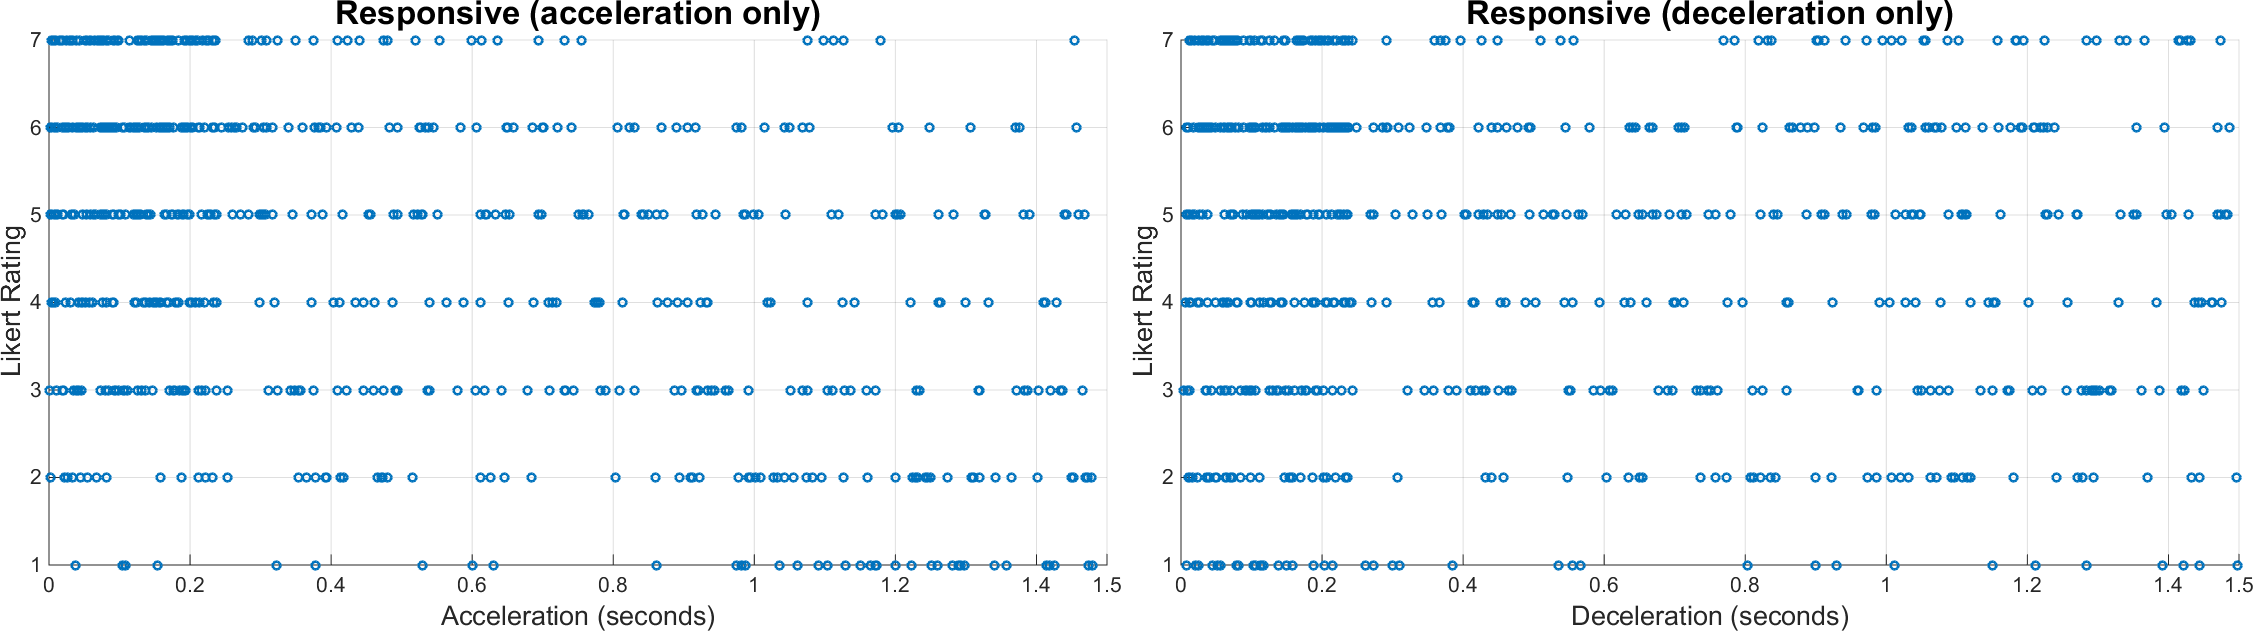
\includegraphics[width=0.95\textwidth]{Pics/Classes/responsive_both}
%\caption{Looking at responsive for acceleration and deceleration.}
%\label{fig:responsive_both}
%\end{figure*}

%\begin{figure}[htbp]
%\centering
%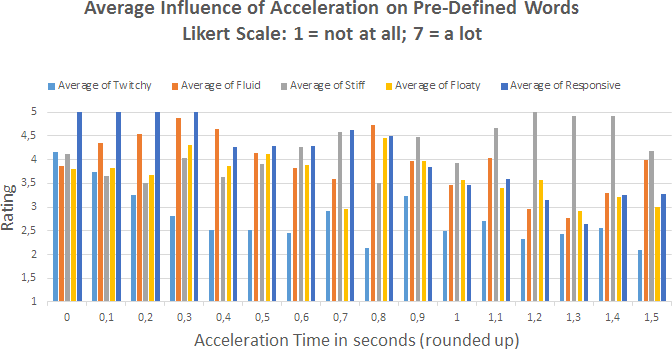
\includegraphics[width=0.97\columnwidth]{Pics/acc_average_response}
%\caption{Average ratings with acceleration.}
%\label{fig:acc_average_response}
%\end{figure}

%\begin{figure}[htbp]
%\centering
%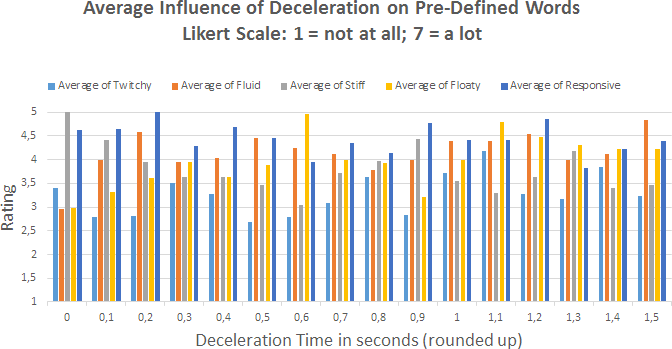
\includegraphics[width=0.97\columnwidth]{Pics/dec_average_response}
%\caption{Average ratings with deceleration.}
%\label{fig:dec_average_response}
%\end{figure}

\begin{figure*}[htbp]
\centering
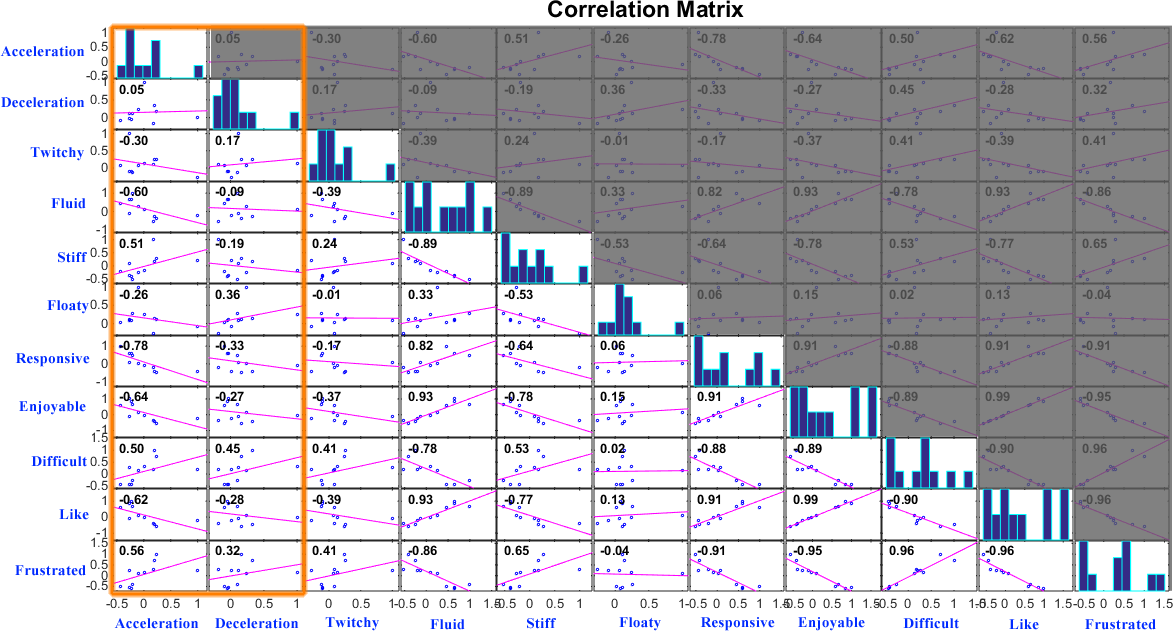
\includegraphics[width=0.98\textwidth]{Pics/correlationMatrix_final}
\caption{Pearson correlation matrix.}
\label{fig:correlationMatrix}
\end{figure*}

\textbf{Looking at Acceleration and Deceleration Simultaneously}\\
The data can also be plotted using acceleration and deceleration simultaneously. The following graphs visualize how the participants rated the game across the different pre-defined words.

Looking at the data, it appears as if the perceived contribution of the acceleration and deceleration values aren't always equal. Generally, there are no strong correlations between the acceleration/deceleration times and the ratings provided by the participants. This might be due to difficulties in understanding and/or interpreting the words. Still, looking at the extremes (1 = \textit{not at all}; 7 = \textit{a lot}), some patterns seem to emerge.

Figure \ref{fig:twitchyFluid} shows  how \textit{twitchy} the game felt. There appears to be one main cluster of 1-ratings. It seems like if the deceleration was low (< 0.2 seconds), participants tended to rate the game less \textit{twitchy}. A similar, yet not as strong, cluster can be seen with low acceleration (< 0.2 seconds) where participants rated the game more \textit{twitchy}. However, due to the uneven sampling (\textit{fast} and \textit{slow} intervals), it is difficult to tell whether this is significant or not.

When it comes to how \textit{fluid} the game felt (Figure \ref{fig:twitchyFluid}), the data suggests that with low deceleration (< 0.1 seconds), the game didn't feel \textit{fluid}. There is also a small cluster of 7-ratings around acceleration/deceleration values between 0.1 and 0.3 seconds.

Figure \ref{fig:stiff_floaty} shows the \textit{stiffness} and \textit{floatyness}. These appear to be inversely proportional to each other, meaning that if both the acceleration and deceleration are low, the game feels more \textit{stiff}, but it also feels less \textit{floaty}. Additionally, there are two clusters with \textit{stiffness}. These present two different interpretations of the word \textit{stiff}. The first is with high acceleration values (> 0.8 seconds), which might mean that the avatar is \textit{stiff} in the sense that it resists change in motion. The other cluster is with lower acceleration values (< 0.3 seconds), where there is an immediate and direct relation between input and avatar motion (similar to Figure \ref{fig:adsr_stiff}). Conversely, with higher deceleration values (> 0.2 seconds), the game doesn't appear very \textit{stiff}.

Figure \ref{fig:stiff_floaty} also shows a slight tendency towards high deceleration values (> 1 second) for a more \textit{floaty} feel.

With \textit{responsiveness}, as shown in Figure \ref{fig:responsive_enjoyable}, there is a clear indication that values below 0.3 seconds appear most \textit{responsive}. That being said, it seems like acceleration have a bigger influence than deceleration, since many participants reported high \textit{responsiveness} even with deceleration values above 0.8 seconds. One possible explanation is the fact that when changing direction (e.g., moving towards left, but suddenly turning towards right), the influence of the deceleration is not as strong, since it, in essence, is overridden by the acceleration in the new direction.

When looking at how \textit{enjoyable} the game felt (see Figure \ref{fig:responsive_enjoyable}), there seems to be a correlation with \textit{responsiveness}, since most participants enjoyed acceleration and deceleration values below 0.3 seconds. The same can be said about how much participants \textit{liked} the controls and how \textit{difficult} the game felt, as shown in Figure \ref{fig:difficult_liked}.

\begin{figure*}[htbp]
\centering
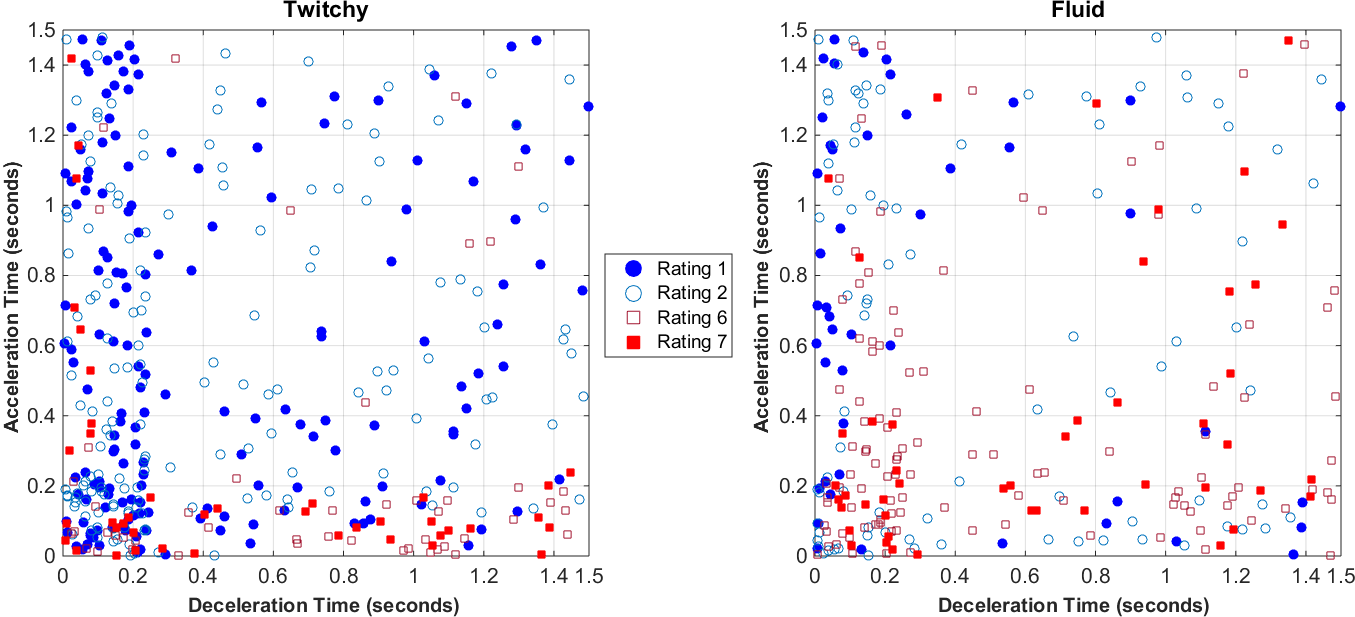
\includegraphics[width=0.67\textwidth]{Pics/Classes/twitchy_fluid}
\caption{Players' self-reported perception on how twitchy and fluid the controls felt, rated using a 7-point Likert scale (only 1, 2, 6 and 7 are shown).}
\label{fig:twitchyFluid}
\end{figure*}

\begin{figure*}[htbp]
\centering
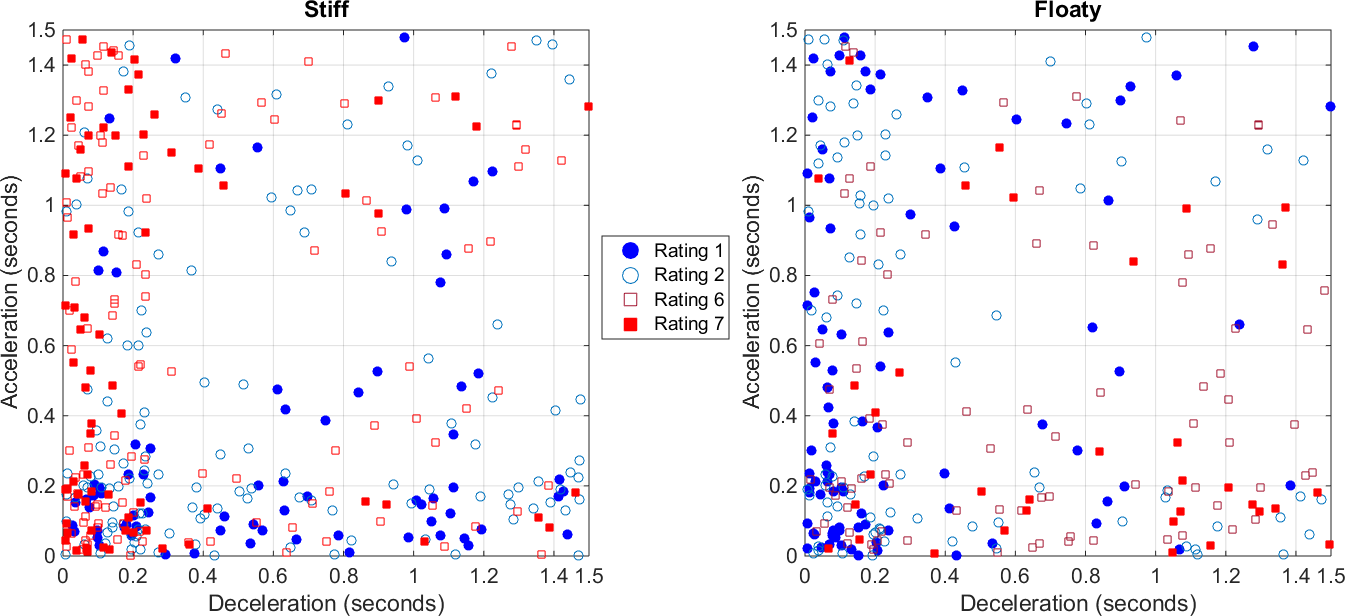
\includegraphics[width=0.67\textwidth]{Pics/Classes/Stiff_floaty}
\caption{Players' self-reported perception on how stiff and floaty the controls felt, rated using a 7-point Likert scale (only 1, 2, 6 and 7 are shown).}
\label{fig:stiff_floaty}
\end{figure*}

\begin{figure*}[htbp]
\centering
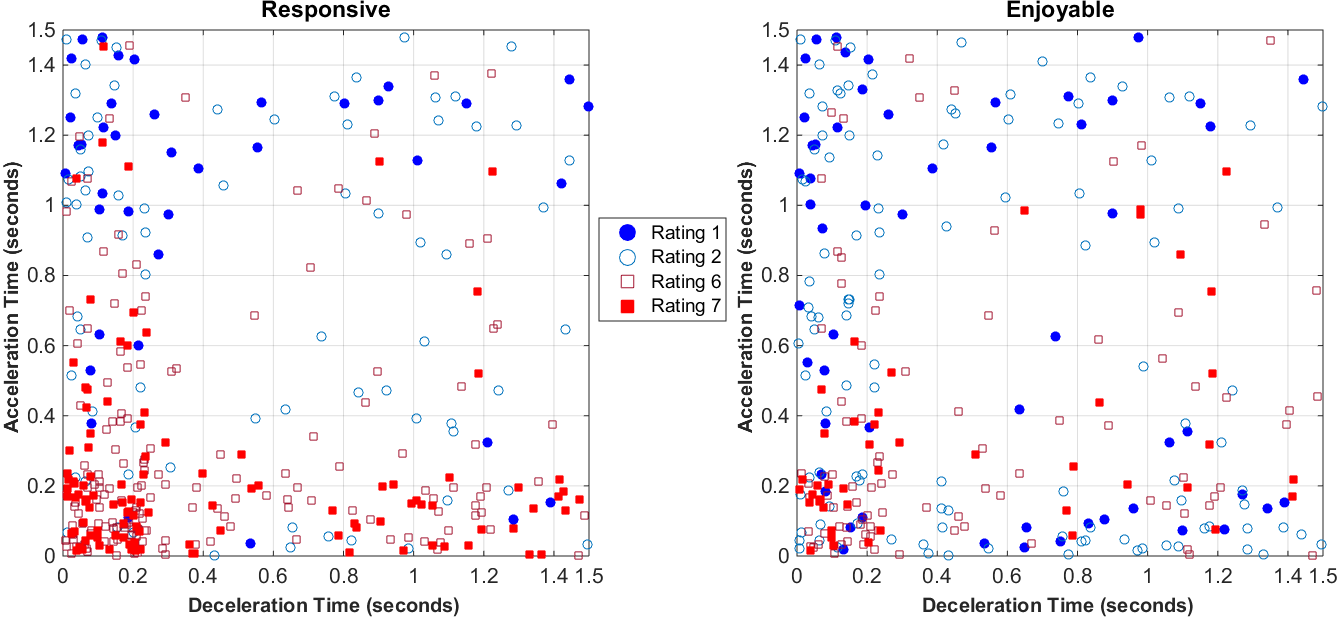
\includegraphics[width=0.67\textwidth]{Pics/Classes/Responsive_enjoyable}
\caption{Players' self-reported perception on how responsive and enjoyable the controls felt, rated using a 7-point Likert scale (only 1, 2, 6 and 7 are shown).}
\label{fig:responsive_enjoyable}
\end{figure*}

\begin{figure*}[htbp]
\centering
\includegraphics[width=0.67\textwidth]{Pics/Classes/difficult_like}
\caption{Players' self-reported perception on how difficult and how much they liked the controls, rated using a 7-point Likert scale (only 1, 2, 6 and 7 are shown).}
\label{fig:difficult_liked}
\end{figure*}

%\begin{figure}[htbp]
%\centering
%\includegraphics[width=0.9\columnwidth]{Pics/Classes/frustrated_alone}
%\caption{Players' self-reported perception on how frustrated they felt the controls were, rated using %a 7-point Likert scale (only 1, 2, 6 and 7 are shown).}
%\label{fig:frustration}
%\end{figure}

\textbf{Looking at Acceleration and Deceleration Simultaneously (Averages)}\\
Since the distribution of the acceleration/deceleration times wasn't equal (due two the two intervals, \textit{fast} and \textit{slow}), a different way to approach the data is to look at averages. In the following plots, the data has been divided into 36 boxes of size 0.25x0.25. The Likert ratings were counted for each of the boxes and then divided by the number of ratings in that particular box, resulting in an overall average. These are shown in Figures \ref{fig:twitchyFluid_avg}, \ref{fig:stiff_floaty_avg}, \ref{fig:responsive_enjoyable_avg}, \ref{fig:difficult_liked_avg} and \ref{fig:frustrated_avg}.

\begin{figure*}[htbp]
\centering
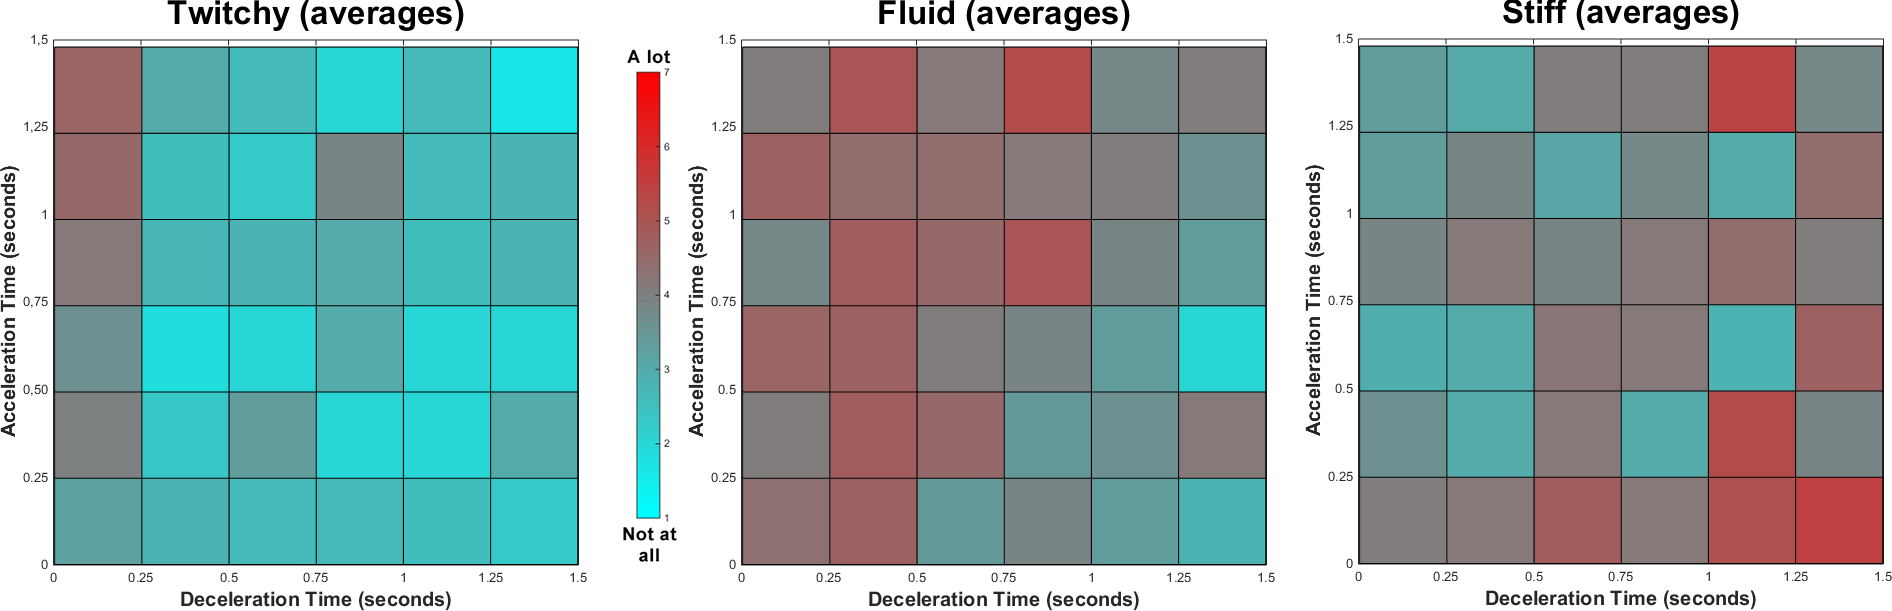
\includegraphics[width=0.67\textwidth]{Pics/Classes/averages/twitchy_fluid_avg}
\caption{Participants' average responses. Each box is 0.25x0.25}
\label{fig:twitchyFluid_avg}
\end{figure*}

\begin{figure*}[htbp]
\centering
\includegraphics[width=0.67\textwidth]{Pics/Classes/averages/Stiff_floaty_avg}
\caption{Participants' average responses. Each box is 0.25x0.25}
\label{fig:stiff_floaty_avg}
\end{figure*}

\begin{figure*}[htbp]
\centering
\includegraphics[width=0.67\textwidth]{Pics/Classes/averages/Responsive_enjoyable_avg}
\caption{Participants' average responses. Each box is 0.25x0.25}
\label{fig:responsive_enjoyable_avg}
\end{figure*}

\begin{figure*}[htbp]
\centering
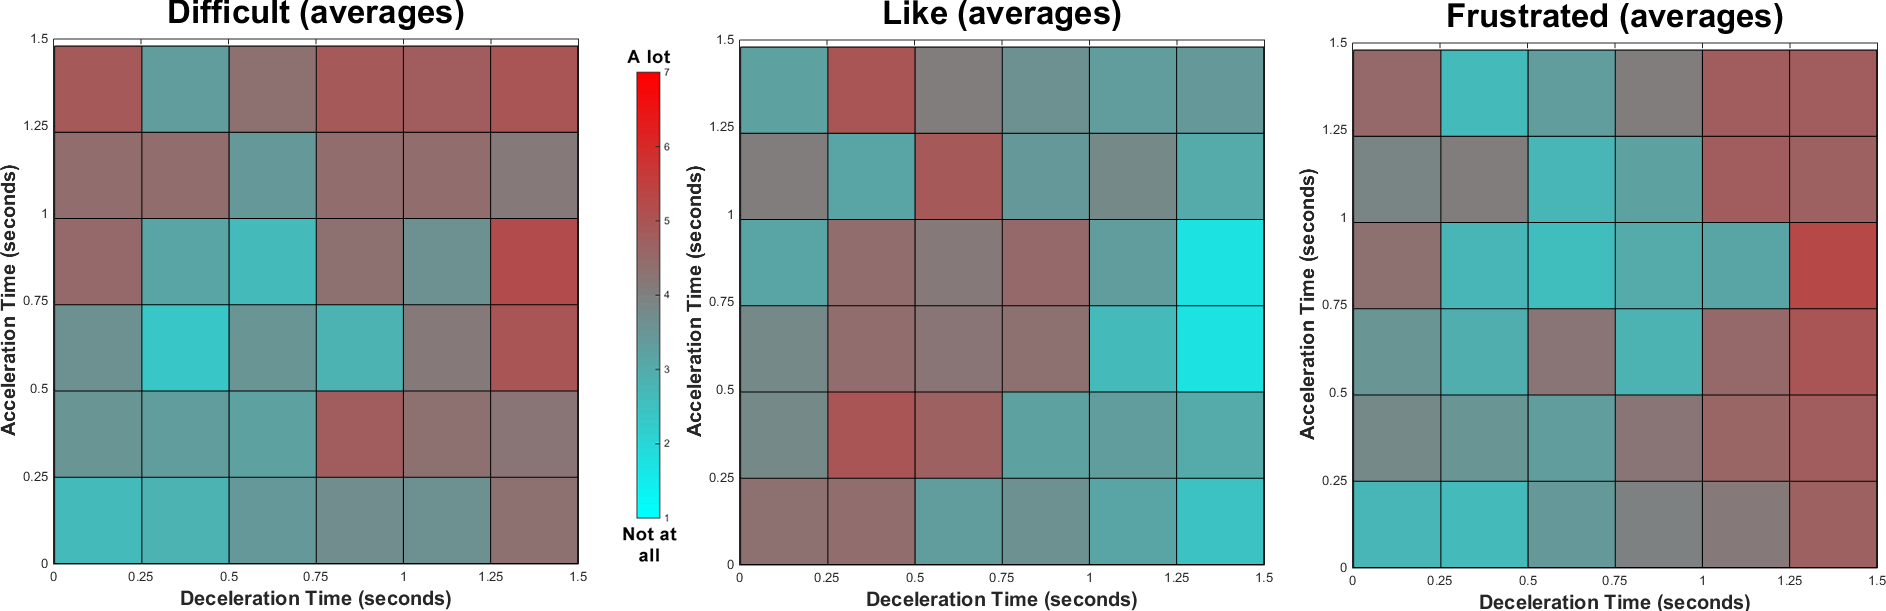
\includegraphics[width=0.67\textwidth]{Pics/Classes/averages/difficult_like_avg}
\caption{Participants' average responses. Each box is 0.25x0.25}
\label{fig:difficult_liked_avg}
\end{figure*}

\begin{figure*}[htbp]
\centering
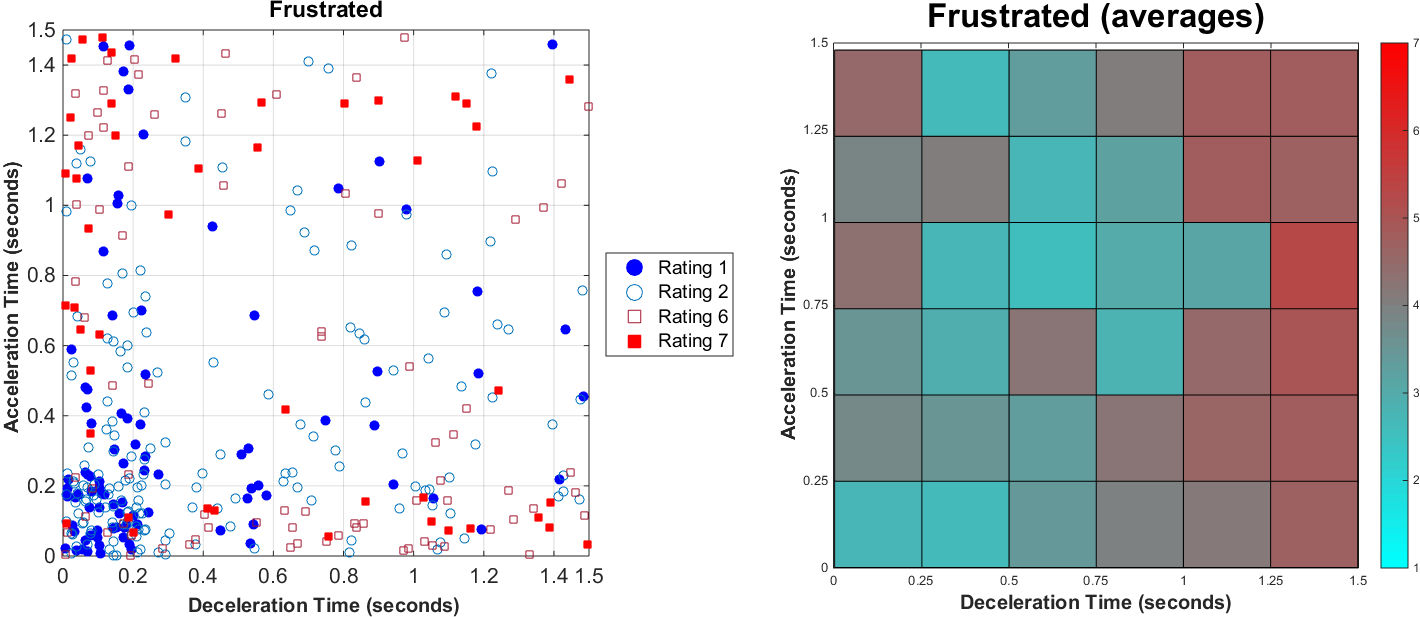
\includegraphics[width=0.67\textwidth]{Pics/Classes/averages/frustrated_frustrated}
\caption{Participants' average responses. Each box is 0.25x0.25}
\label{fig:frustrated_avg}
\end{figure*}

\textbf{Curves}\\
Yet another way to visualize the data is to take the averages of the acceleration/deceleration values for each of the ratings, e.g., the average acceleration/deceleration values for \textit{twitchy} rating 1, rating 2, rating 3, etc. However, since a Likert scale consists of ordinal values, there is no guarantee that a rating difference of 1 represents an equal conceptual change, since the scale might be used differently by different participants. For instance, some participants might be hesitant to use the extreme values 1 (\textit{not at all}) and 7 (\textit{a lot}), while others might spread their answers across the whole scale \cite{cunningham}. Because of this, in the following graphs, the averages have been put into three weighted categories, so that the extreme ends contribute more. The \textit{low rating} curves consist of ratings 1 (70\%), 2 (20\%) and 3 (10\%). The \textit{mid rating} curves consist of ratings 3 (25\%), 4 (50\%) and 5 (25\%). The \textit{high rating} curves consist of ratings 5 (10\%), 6 (20\%) and 7 (70\%). Using these numbers, it is now possible to draw acceleration/deceleration curves, as seen in Figures \ref{fig:curve_twitchy}, \ref{fig:curve_fluid}, \ref{fig:curve_stiff}, \ref{fig:curve_floaty} and \ref{fig:curve_responsive}. For all curves, the sustain time is 1 second. The numbers in square brackets represent acceleration and deceleration values.

At first glance, many of the curves seem similar. However, when comparing the three curves from the same word, there are some differences. For instance, there is a difference of about 360 milliseconds between the deceleration in \textit{low rating} and \textit{high rating} in the \textit{floaty}. curve. Also, it should be noted that the different curves are not mutually exclusive, i.e., the controls can feel \textit{floaty} and \textit{fluid} at the same time.

\begin{figure}[htbp]
\centering
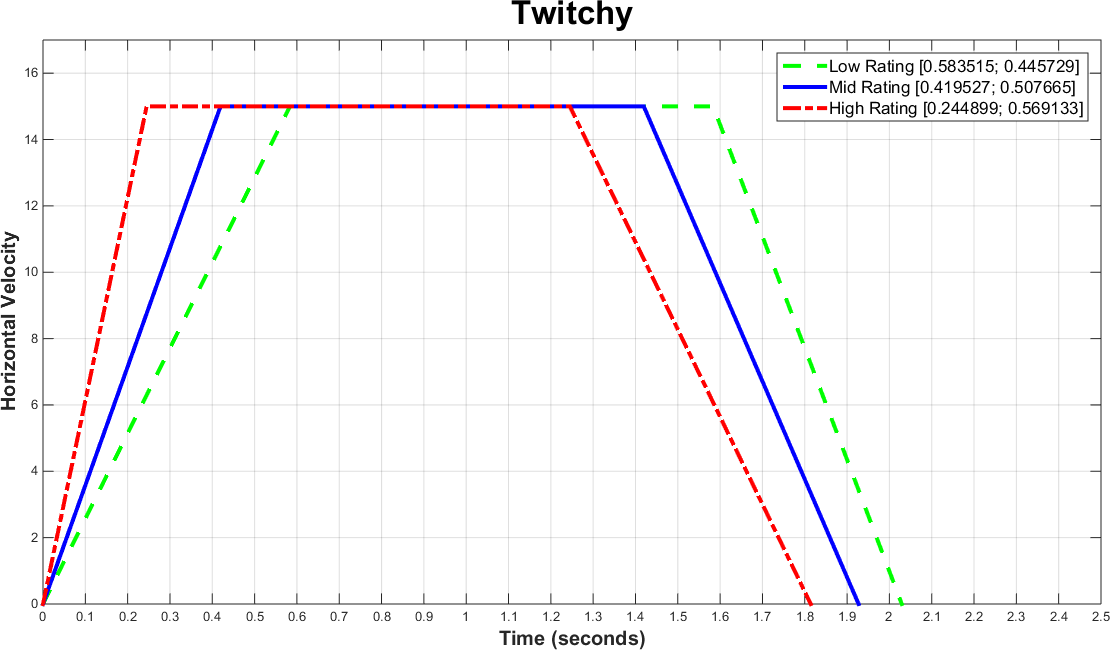
\includegraphics[width=0.9\columnwidth]{Pics/Curves/Twitchy_curve}
\caption{Average curves of twitchy controls.}
\label{fig:curve_twitchy}
\end{figure}

\begin{figure}[htbp]
\centering
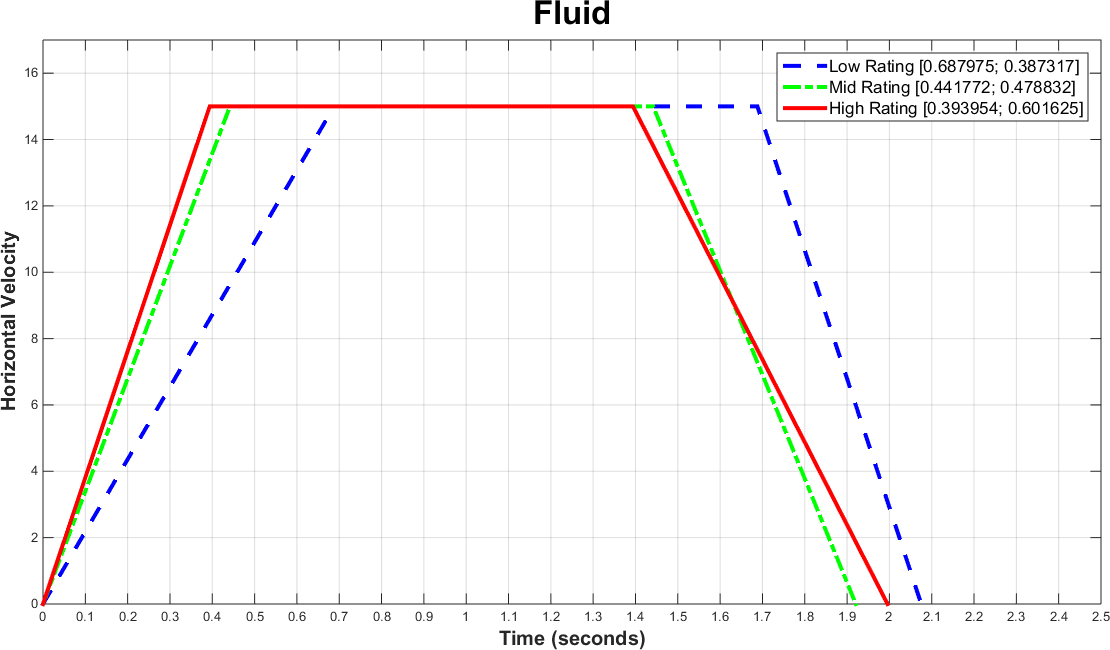
\includegraphics[width=0.9\columnwidth]{Pics/Curves/Fluid_curve}
\caption{Average curves of fluid controls.}
\label{fig:curve_fluid}
\end{figure}

\begin{figure}[htbp]
\centering
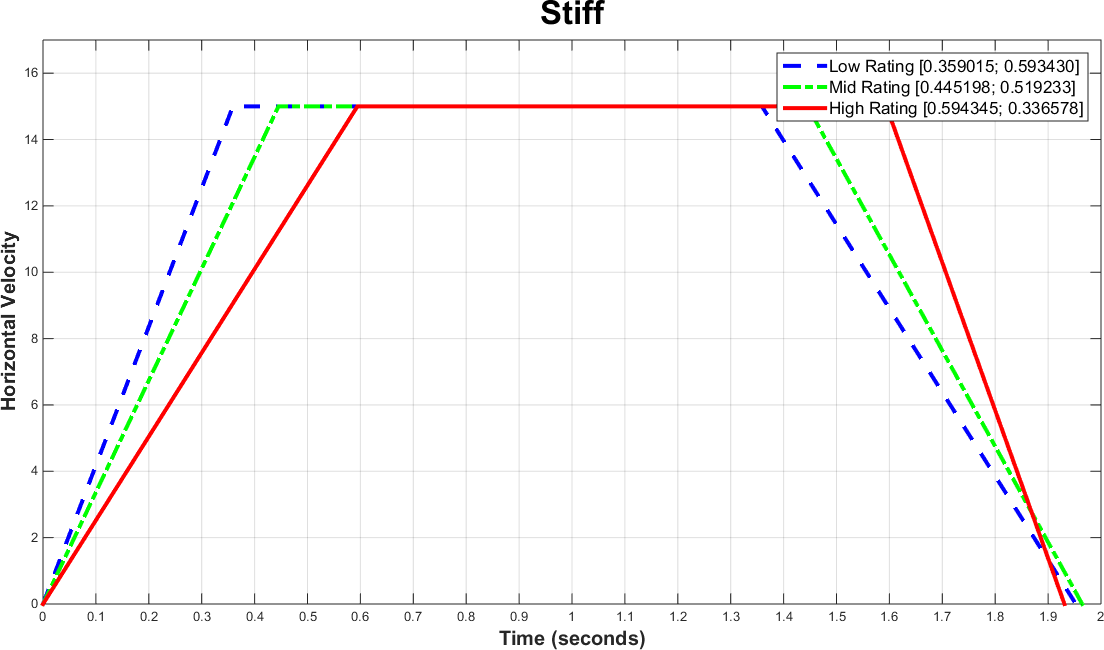
\includegraphics[width=0.9\columnwidth]{Pics/Curves/Stiff_curve}
\caption{Average curves of stiff controls.}
\label{fig:curve_stiff}
\end{figure}

\begin{figure}[htbp]
\centering
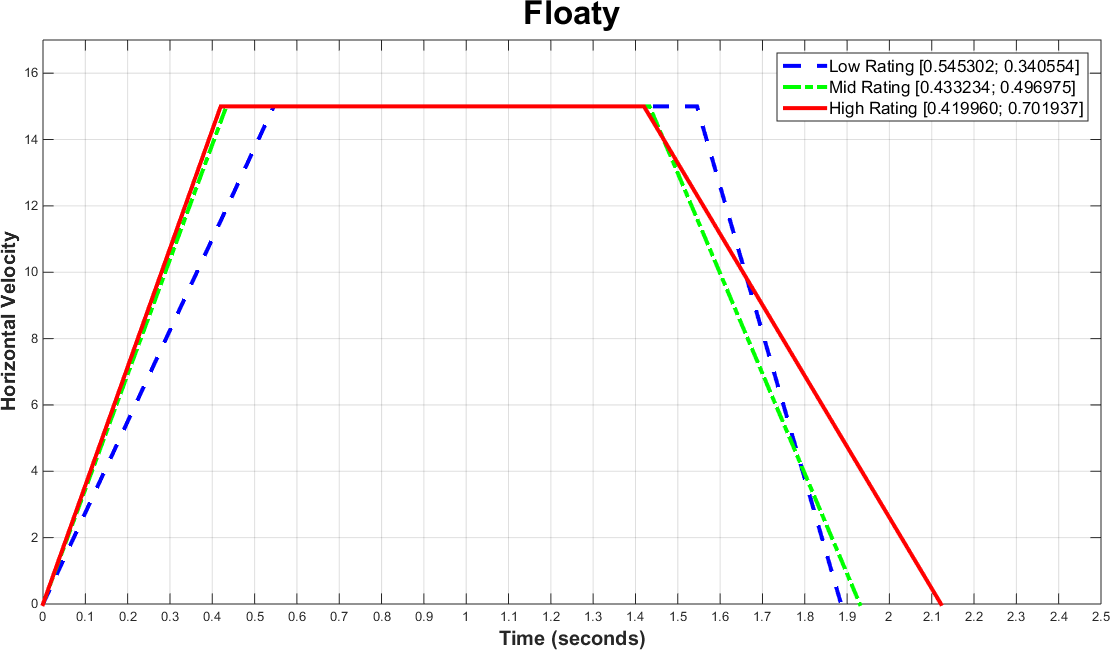
\includegraphics[width=0.9\columnwidth]{Pics/Curves/Floaty_curve}
\caption{Average curves of floaty controls.}
\label{fig:curve_floaty}
\end{figure}

\begin{figure}[htbp]
\centering
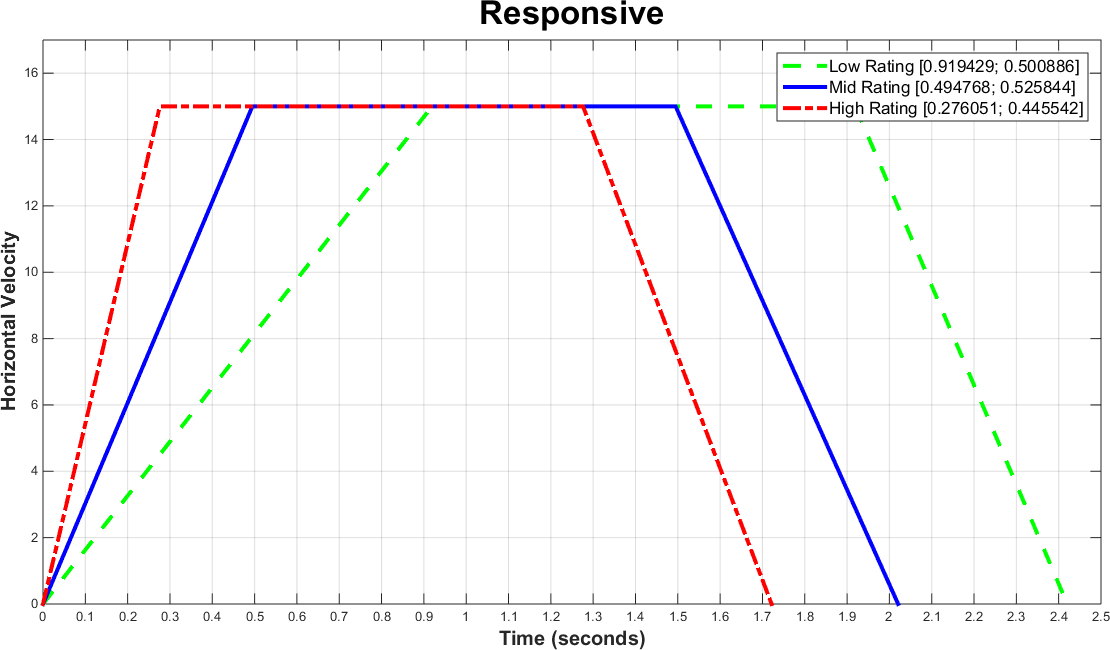
\includegraphics[width=0.9\columnwidth]{Pics/Curves/Responsive_curve}
\caption{Average curves of responsive controls.}
\label{fig:curve_responsive}
\end{figure}

\subsection{Post-questionnaire}
After completing the fourth round of the game, participants were asked to complete a Google Forms questionnaire. At the time of writing, 153 participants have taken part in this post-questionnaire. Participants were asked to answer the following questions, as well as describing the feel of six other 2D platforming games.
\begin{itemize}[noitemsep,nolistsep]
\item What parameters do you think changed between each round in the ball game?
\item Name one game you think feels good (different from the ball game you just played)
\item In your own words, how would you define the feel of games?
\item In general, how important do you find the feel of games?
\item How would you describe the feel of each of the following games/series?
\begin{itemize}[noitemsep,nolistsep]
\item Mega Man
\item LittleBigPlanet
\item Donkey Kong
\item Super Meat Boy
\item Prince of Persia (1989)
\item Super Mario Bros.
\end{itemize}
\end{itemize}

\begin{figure}[htbp]
\centering
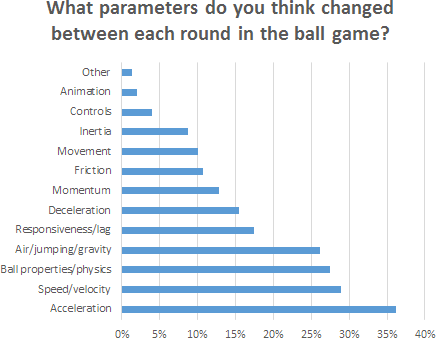
\includegraphics[width=0.9\columnwidth]{Pics/whatChanged}
\caption{What the participants thought changed between rounds.}
\label{fig:whatChanged}
\end{figure}

\begin{figure}[htbp]
\centering
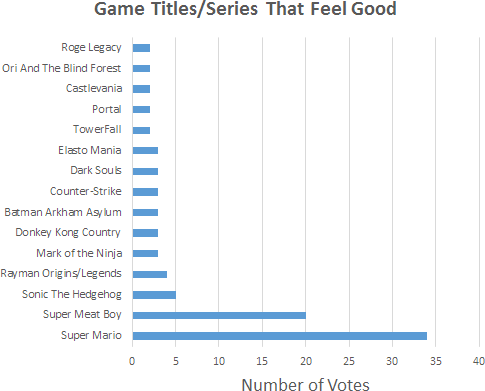
\includegraphics[width=0.9\columnwidth]{Pics/good_games}
\caption{Game titles/series that the participants though feel good. Only those with more than one vote are included.}
\label{fig:good_games}
\end{figure}

\begin{table} \centering
\caption{The 30 most commonly-used words to define game feel in the post-questionnaire (among the 153 data entries). Numbers in parenthesis indicate usage frequency. Common grammar words have been excluded. Words with duplicate entries such as \textit{games} and \textit{game} have been combined into one.}
\label{table:mostWordsPost_GF}
\begin{tabular}{lll}
\toprule
game (193) & feel (160) & control (87)\\
how (46) & like (42) & player (34)\\
good (26) & way (23) & character (22)\\
really (18) & too (18) & something (17)\\
should (17) & me (17) & play (16)\\
gameplay (13) & responsive (13) & don't (13 times)\\
get (13) & question (12) & easy (11)\\
world (11) & bad (11) & responsiveness (11)\\
will (11) & between (10) & actions (10)\\
time (10) & important (10) & playing (9)\\
\bottomrule
\end{tabular}
\end{table}

\begin{table} \centering
\caption{The 30 most commonly-used words to describe six other platform games in the post-questionnaire (among the 153 data entries). Numbers in parenthesis indicate usage frequency. Common grammar words have been excluded. Words with duplicate entries such as \textit{games} and \textit{game} have been combined into one.}
\label{table:mostWordsPost}
\begin{tabular}{lll}
\toprule
game (252) & feel (214) & control (209)\\
very (134) & played (97) & responsive (85)\\
like (81) & jump (63) & never (58)\\
fast (57) & character (57) & good (56)\\
really (53) & mario (51) & great (50)\\
slow (49) & floaty (47) & because (46)\\
time (46) & too (45) & fun (45)\\
just (43) & bit (42) & movement (41)\\
precise (41) & hard (41) & super (40)\\
jumping (40) & jumps (36) & frustrating (35)\\
\bottomrule
\end{tabular}
\end{table}

Figure \ref{fig:whatChanged} shows what the participants thought had changed between the rounds. Even though only acceleration and deceleration changed, participants also perceived other changes as well, most notably changes about how the controls felt in the air, such as how gravity and jumping worked. This might partially be due to the variable jump that some players may have missed in the first few rounds. Some also focused on the ball's properties, such as its mass and how ``ball-like" it behaved. In regards to acceleration and deceleration, more than double as many mentioned acceleration. When looking at the responses, it seems like participants were unaware of the term \textit{deceleration}, often times talking about how the ball gradually would slow down to a halt.

Figure \ref{fig:good_games} shows the games that the participants think feel good. Even though the question was phrased as \textit{Name one game you think feels good (different from the ball game you just played)}, many thought that they should name a 2D platforming game.

Table \ref{table:mostWordsPost_GF} shows the 30 most-commonly used words that participants used when trying to answer the question \textit{In your own words, how would you define the feel of games?}

Table \ref{table:mostWordsPost} shows the 30 most commonly-used words that participants used to describe the feel of the six 2D platforming games. Below are some selected quotes for describing the feel of each of the games (some quotes have been combined for the sake of clarity).
\textbf{Mega Man (1987)}
\vspace{-5mm}
\begin{itemize}[noitemsep,nolistsep]
\item Very responsive and you feel in control in general. It does lack on game feel though, because some jumps require pixel-perfect positioning which makes you think actively about mechanics.
\item Stiff, rigid, bland, cold, futuristic, direct and robotic.
\item It isn't fast and fluid like Super Meat Boy, you feel more like a robot in a heavy armored suit, but the feel is still perfectly paired with it's level and enemy design.
\item The controls in Mega Man are very slow and floaty. However, the game is based around moving slowly and attacking from a distance. The jumping is floaty, yet responsive to player inputs, such as changing direction in midair, or stopping the jump early. 
\item Responsive, since Mega Man moves when you press the button, and stops when you don't. The game, however, sometimes feels a bit clunky since you can only shoot straight, but the level design makes up for this most of the time.
\item Very solid ground and air control. You have proper air control and Mega Man doesn't stop at the exact moment you let go of the d-pad. He slides a few pixels further, which feels natural.
\item Super tight, super retro, no wiggle room. The fact that Mega Man stops completely when you let go of the button takes a bit of getting used to, but allows for precision in ways you wouldn't expect. Our brains are wired for natural physical projectile motion (IE parabolic), but Mega Man forces you to ignore that, which takes some getting used to.
\item Feels very flat, the controls are too tight for proper game feel.
\end{itemize}

\textbf{LittleBigPlanet (2008)}
\vspace{-5mm}
\begin{itemize}[noitemsep,nolistsep]
\item Incredibly floaty to the point where it just isn't enjoyable. It feels like you have NO control over the character.
\item Floaty and squishy, inertia-based - character has sense of inertia - height and length of jumps are determined by speed of character movement and button press duration. Jumps are slow and floaty etc
\item Nice and fluid. Sort of "organic". Everything moves naturally according to things like gravity, force-impact, etc.
\item Just terrible to control. Everything about the controls is too floaty, making precise jumping a chore. A lot could have been improved by enabling D-pad controls, as the analog sticks tend to increase the floaty feel, and it's generally much more imprecise for this type of game.
\item Game is very responsive but the control schemes are convoluted and overly complicated. 
\item Laid back and relaxed. It's fun and easy, it's responsive and the controls are pretty straightforward.
\item Floaty and with inertia controls. The slightly imprecise nature of the platforming makes for interesting mistakes to occur when playing with friends, but it is not so egregious that it is game breaking. 
\item On ground the game has a brilliant feel. It has the perfect speed and momentum. In air I found this game very frustrating.
\item Child-like. Super happy. The animations really make a huge difference in how this game feels.
\end{itemize}

\textbf{Donkey Kong (1981)}
\vspace{-5mm}
\begin{itemize}[noitemsep,nolistsep]
\item A bit sluggish, lends either a feeling of panic or frustration to me depending on whether I win or lose. Mario feels a bit difficult to control, the jumps are hard to gauge and he never seems to move quite quickly enough. It feels like slogging through a chest-high swamp.
\item Good decent controls. It's very precise with no room for errors. But completely lacks any kind of air control. Mario is definitely floaty, but with almost slow-motion jump physics.
\item Mario feels responsive on the ground, if a bit slow, but his jumping feels far too floaty, and he's locked into his jumping trajectory, which almost never works in a game centered around jumping over obstacles and pits.
\item Squarish - hard to explain.
\item Direct, unforgiving, repetitive, snappy.
\item Precise and sloppy. Two words wide from each other, but it's the best I can describe it. It requires precision to jump the barrels, and the controls and overall feel provides that, but in the same time, it doesn't feel like you got much else control of Mario.
\item Clunky, odd hitboxes and arcade-like. Twitchy, inflexible, stiff, light.
\item Frustrating. The timing required for everything is so precise that even beating a single level is a challenge.
\end{itemize}

\textbf{Super Meat Boy (2010)}
\vspace{-5mm}
\begin{itemize}[noitemsep,nolistsep]
\item Awesome. Smooth and fast-paced movement that requires skill. Very good acceleration and deceleration of the character. The air control feels natural and is influenced greatly by the characters momentum. 
\item Fluid, precise, controlled, reactive, tight, streamlined.
\item Very twitchy and quick, but wasn't hard to maintain control. The control over Meat Boy is so total that it's very easy to mess up at any point even when you're very close to doing the right thing, and his movement speed and acceleration are high enough that you need to react very fast.
\item Raw, brutal, unforgiving, sarcastic, energetic.
\item Meat Boy is slidey on the ground, but sticks to the walls, making the wall jumps almost like beats in the rhythm of the game. Responsive, slippery but consistent.
\item Fun because the controls are very easy to use and learn. And very intuitive too. Also the graphics sound/aesthetics match the game and the controls very well somehow.
\item Free, fluid, unstoppable, flowing, sloppy. Smooth and comfortable.
\item Massively floaty. The controls are often hailed as "tight", but that only seems to come from the responsiveness, not the actual movement physics, which are very floaty and unpredictable.
\item Part of the game feel is sound design. In Meat Boy, you see him run up to speed, and as he gets faster you hear his little wet footsteps. It's rewarding to the player to get that feedback, it makes you FEEL fast. If Meat Boy was a red featureless square with no sound, it'd be a vastly inferior 'feeling' game.
\item It's often praised for having tight controls, but in my opinion, they're a bit loose. For the most part you feel in control.
\end{itemize}

\textbf{Prince of Persia (1989)}
\vspace{-5mm}
\begin{itemize}[noitemsep,nolistsep]
\item Super limited. Static animations, no chance of survival. It's more of a strategy game than a platformer, honestly.
\item Old and mushy. You can't really control your character easily (jumps, moves, etc.), and the controls don't feel responsive.
\item The controls are very difficult to master because when you stop pressing a button the prince will still be moving, and therefore it is very hard to time you jump. One of the rounds in your game had the same kind of feel.
\item Controls are responsive, but the movement is completely unpredictable due to the environment seemingly actually affecting the velocity and acceleration of the character, where it normally would just intervene in other games. More apparent rules for the character's steps or jump lengths would help tighten the game feel, but as it stands, it's very weighty and unpredictable.
\item Slow, imprecise and sloppy as hell. You would have to play around the controls, and have it in mind all the time.
\item Quite unstable. You are never sure whether what you are doing will result in the wished action. Jumping seems rather hit and miss.
\item Prince of Persia was absolutely amazing when it came out. The body dynamics were unlike anything I'd seen in a computer game before. It was sometimes hit-and-miss with the timing of jumps, but overall very responsive.
\item Delayed responsiveness and a little twitchy. You're never quite sure where the character's hitbox actually is, making jumping very frustrating.
\item Great controls. Tight and a yet a good sense of weight behind the character.
\item Adventurous. Unforgiving, slippery.
\item Squarish and clunky, but also very responsive... but in a weird sort of unresponsive way
\item Deliberate, heavy, cumbersome, delayed, planned. 
\end{itemize}

\textbf{Super Mario Bros. (1985)}
\vspace{-5mm}
\begin{itemize}[noitemsep,nolistsep]
\item It feels very responsive. Actions are quick and takes zero effort to master.
\item Fast and loose.
\item The movement is a bit clunky since Mario slides around, but its okay since the game doesn't have many big precise jumps.
\item Smooth, strange and foreign, also classic.
\item Floaty, awkward jumping and running. Momentum really holds and it feels like you are piloting a brick.
\item Tight, predictable acceleration and momentum velocities. Instantly responsive controls, and although the character portrays a lot of acceleration and momentum after having stopped, it's always the same, becoming predictable and thus, enjoyable.
\item A bit draggy - slow acceleration and long jump time.
\item Fairly responsive but a bit twitchy because Mario's movement in midair is difficult to control. The capacity to run by pressing one button is clever as it provides a better move control for difficult parts.
\item Very swift, easy to control, rewarding.
\item Simple and predictable. No stress. You can focus on tasks instead of the controls.
\item Great overall feel which is why it was/is so popular. The run button pretty much allowed you to switch between two separate feels, one slow and one fast.
\item Slow to accelerate, but the levels are designed around it. Top speed is fast, jump arc is nice (the top of it is weird, he hangs there a bit, outside of a standard arc). Basically, Mario gives you the freedom to go slow or fast, and provides enough wide open space for it to feel good.
\item Perfectly middle-of-the-pack in terms of physics. A little bit slippery and a little bit floaty, but not noticeably so in either category.
\end{itemize}

As the above quotes show, players tend to focus on different elements when it comes to game feel. What feels `unresponsive' and `floaty' to some may feel more responsive and relaxed to others. It all depends on the context of use, as one participant expressed when describing the feel of \textit{LittleBigPlanet}. If playing in a casual/social setting, it might not matter that the feel is `floaty' and `imprecise': \textit{``The slightly imprecise nature of the platforming makes for interesting mistakes to occur when playing with friends"}. It all comes down to what type of game it is and how challenging it's supposed to be. For instance, one participant described the feel of \textit{Super Mario Bros.} to be `clunky', but found it acceptable, since the game doesn't feature many big and precise jumps.

Some also mentioned the usage of animation and sound effects, which again confirms that game feel is about the overall player perception. In general, as shown in Figure \ref{fig:games_important}, most participants find the feel of games very important.

\begin{figure}[htbp]
\centering
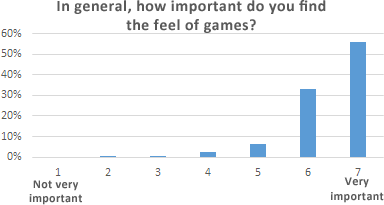
\includegraphics[width=0.9\columnwidth]{Pics/games_important}
\caption{Participants found game feel to be quite important.}
\label{fig:games_important}
\end{figure}